%%% Copyright (C) 2017 Vincent Goulet
%%%
%%% This file and all files included or input by this one (and
%%% recursively) are part of the project "A foray into the Insurance
%%% of Things, Or pricing individual objects without prior data - IME
%%% 2017"
%%% http://github.com/vigou3/ime-2017-insurance-of-things
%%%
%%% This work is licensed under a Creative Commons
%%% Attribution-ShareAlike 4.0 International License.
%%% http://creativecommons.org/licenses/by-sa/4.0/

\documentclass[aspectratio=1610,10pt,xcolor=x11names]{beamer}
  \usepackage[round]{natbib}             % references
  \usepackage{fontawesome}               % various icons
  \usepackage{changepage}                % page licence
  \usepackage{tabularx}                  % page licence
  \usepackage{framed}                    % env. leftbar
  \usepackage[export]{adjustbox}         % cadre autour image
  \usepackage[overlay,absolute]{textpos} % covers
  \usepackage{metalogo}                  % logo \XeLaTeX
  \usepackage{actuarialsymbol}           % symbols in One More Thing

  %% ==================
  %%  Publication info
  %% ==================
  \renewcommand{\year}{2017}

  %% ===============================
  %%  Look and feel of the document
  %% ===============================

  %% Beamer theme
  \usetheme{metropolis}

  %% Math in sans serif font
  \usepackage[frenchmath,scaled=1.15]{newtxsf}

  %% Additionnal colors
  \definecolor{link}{rgb}{0,0.4,0.6}        % internal links
  \definecolor{url}{rgb}{0.6,0,0}           % external links
  \definecolor{rouge}{rgb}{0.85,0,0.07}     % UL red stripe
  \definecolor{or}{rgb}{1,0.8,0}            % UL yellow stripe
  \colorlet{alert}{mLightBrown} % alias for Metropolis color
  \colorlet{dark}{mDarkTeal}    % alias for Metropolis color

  %% Hyperlinks
  \hypersetup{%
    pdfauthor = {Vincent Goulet},
    pdftitle = {A foray into the Insurance of Things, Or pricing%
      individual objects without prior data},
    colorlinks = {true},
    linktocpage = {true},
    allcolors = {link},
    urlcolor = {url},
    pdfpagemode = {UseOutlines},
    pdfstartview = {Fit},
    bookmarksopen = {true},
    bookmarksnumbered = {true},
    bookmarksdepth = {subsection}}

  %% Bibliography
  %% Couple of hacks needed to have beamer and natbib play nice with
  %% each other.
  \renewcommand{\newblock}{}    % https://tex.stackexchange.com/a/1971/24355
  \renewcommand{\bibsection}{}  % drop \section heading
  \bibliographystyle{abbrvnat}

  %% ===============================
  %%  New commands and environments
  %% ===============================

  %% Theorem-like environments
  \theoremstyle{plain}
  \newtheorem{assumption}{Assumption}
  \theoremstyle{definition}
  \newtheorem{consequence}{Consequence}

  %% Link to GitHub on copyright page
  \newcommand{\viewsource}[1]{%
    \href{#1}{%
      \makebox[2.5mm]{\raisebox{-1pt}{\footnotesize\faGithub}}\;%
      {View on GitHub}}}

  %% single entry for symbol and shortcut lists
  %% http://tex.stackexchange.com/a/128441
  \usepackage{xparse}
  \ExplSyntaxOn
  \NewDocumentCommand{\rshowcase}{v} { \texttt{#1} & \tl_rescan:nn { } { $#1$ } }
  \ExplSyntaxOff

  %% Context-specific commands
  \newcommand{\esp}[1]{E [ #1 ]}
  \newcommand{\VaR}{\ensuremath{\text{VaR}}}
  \newcommand{\TVaR}{\ensuremath{\text{TVaR}}}
  \newcommand{\feu}{{[\text{F}]}}
  \newcommand{\eau}{{[\text{W}]}}
  \newcommand{\bris}{{[\text{A}]}}
  \newcommand{\DOT}{{[\ast]}}

  %%% =======
  %%%  Varia
  %%% =======

  %% Lengths used to compose front and rear covers.
  \newlength{\banderougewidth} \newlength{\banderougeheight}
  \newlength{\bandeorwidth}    \newlength{\bandeorheight}
  \newlength{\imageheight}     \newlength{\imagewidth}
  \newlength{\logoheight}
  \newlength{\gapwidth}

%  \includeonly{licence}

\begin{document}

%% frontmatter
\begingroup

\TPGrid{3}{36}
\textblockorigin{0mm}{0mm}
\setlength{\parindent}{0mm}
\setlength{\banderougewidth}{2\TPHorizModule}
\setlength{\banderougeheight}{\TPVertModule}
\setlength{\bandeorwidth}{\TPHorizModule}
\setlength{\bandeorheight}{\banderougeheight}
\setlength{\imageheight}{29\TPVertModule}
\setlength{\imagewidth}{3\TPHorizModule}
\setlength{\logoheight}{2.5\TPVertModule}
\setlength{\gapwidth}{0.75pt}
\addtolength{\bandeorwidth}{-\gapwidth}
\addtolength{\imageheight}{-\gapwidth}

\begin{frame}[plain]
  %% UL banner
  \begin{textblock*}{3\TPHorizModule}[0,1](0mm,30\TPVertModule)
    \textcolor{rouge}{\rule{\banderougewidth}{\banderougeheight}}% % red stripe
    \rule{\gapwidth}{0pt}%                                         % gap
    \textcolor{or}{\rule{\bandeorwidth}{\bandeorheight}}           % gold stripe
  \end{textblock*}

  %% UL logo
  \begin{textblock*}{\TPHorizModule}(2\TPHorizModule,31\TPVertModule)
    \rule{\gapwidth}{0pt}%                                     % gap
    \includegraphics[height=\logoheight,keepaspectratio=true]{ul_p}
  \end{textblock*}

  %% background image
  \begin{textblock*}{3\TPHorizModule}(0mm,0mm)
    %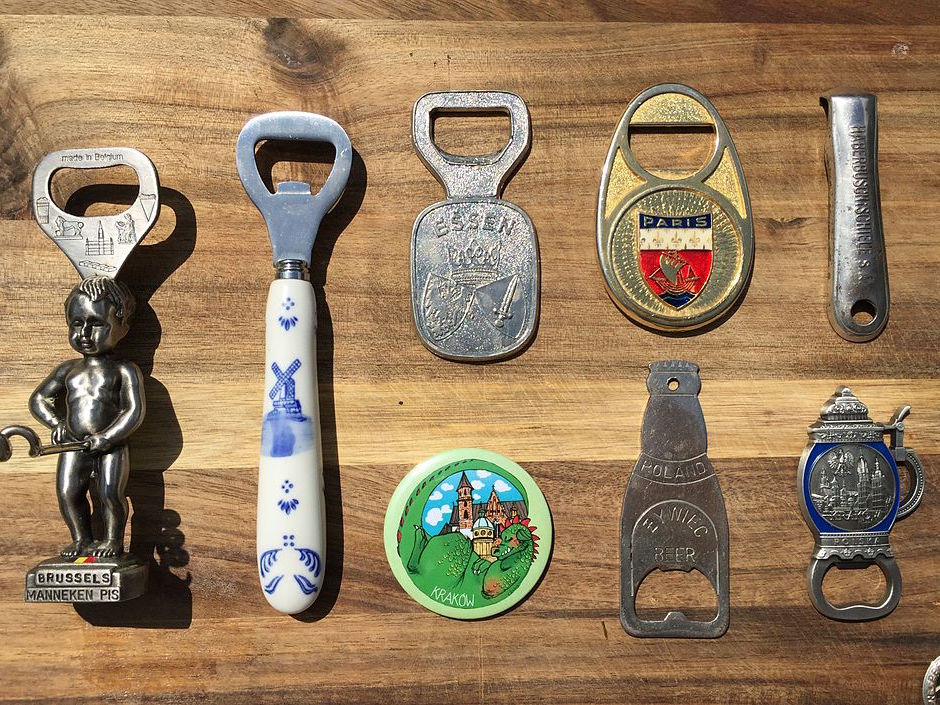
\includegraphics[height=\imageheight,width=\imagewidth]{Collection_of_bottle_openers}
    %\includegraphics*[height=\imageheight,width=\imagewidth]{Match_and_match_labels,_100_years_ago}
    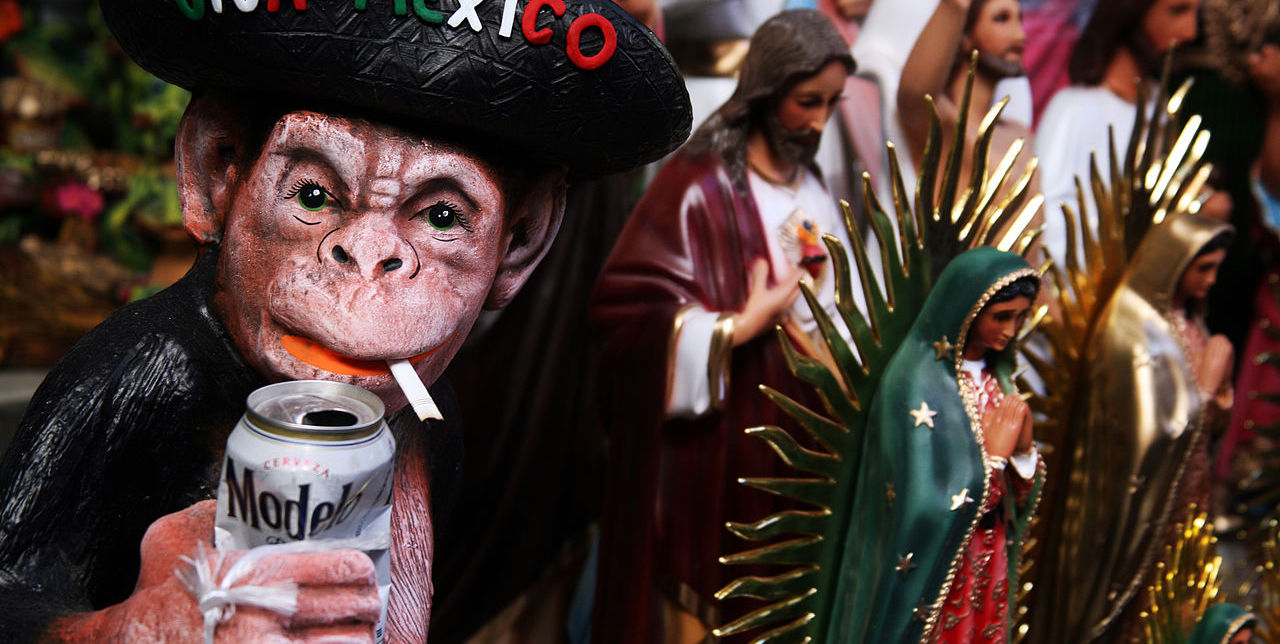
\includegraphics[height=\imageheight,width=\imagewidth]{1280px-Mexican_curious_monkey}
  \end{textblock*}

  %% title
  \begin{textblock*}{2.5\TPHorizModule}(0.205\TPHorizModule,12.1\TPVertModule)
    %% Poor Man's (but simple!) shadow effect behind letters; needed
    %% to let the title stand out on the dark background
    \raggedright%
    \bfseries
    \fontsize{20}{20}\selectfont
    \textcolor{black}{%
      A foray into the Insurance of Things, \\
      Or pricing individual objects \\
      without prior data} \\
    \mdseries
    \fontsize{12}{13}\selectfont
    \textcolor{black}{%
      21\textsuperscript{st} International Congress on
      Insurance: \\ Mathematics and Economics \\
      July 3--5, 2017}
  \end{textblock*}
  \begin{textblock*}{2.5\TPHorizModule}(0.2\TPHorizModule,12\TPVertModule)
    \raggedright%
    \bfseries
    \fontsize{20}{20}\selectfont
    \textcolor{white}{%
      A foray into the Insurance of Things, \\
      Or pricing individual objects \\
      without prior data} \\
    \mdseries
    \fontsize{12}{14}\selectfont
    \textcolor{white}{%
      21\textsuperscript{st} International Congress on
      Insurance: \\ Mathematics and Economics \\
      July 3--5, 2017}
  \end{textblock*}
\end{frame}
\endgroup

%%% Local Variables:
%%% mode: latex
%%% TeX-engine: xetex
%%% TeX-master: "ime-2017-insurance-of-things"
%%% End:

\begingroup

\TPGrid{3}{36}
\textblockorigin{0mm}{0mm}
\begin{frame}[plain]
  %% author
  \begin{textblock*}{2\TPHorizModule}(0.2\TPHorizModule,4\TPVertModule)
    \fontsize{12}{12}\selectfont
    \bfseries
    Vincent Goulet \\
    \fontsize{10}{11}\selectfont
    \mdseries
    École d'actuariat, Université Laval
  \end{textblock*}

  %% title
  \begin{textblock*}{2.5\TPHorizModule}(0.2\TPHorizModule,12\TPVertModule)
    \raggedright%
    \bfseries
    \fontsize{20}{20}\selectfont
    A foray into the Insurance of Things, \\
    Or pricing individual objects \\
    without prior data \\
    \mdseries
    \fontsize{12}{13}\selectfont
    21\textsuperscript{st} International Congress on
    Insurance: \\ Mathematics and Economics -- IME 2017 \\
    July 3--5, 2017
  \end{textblock*}
\end{frame}
\endgroup

%%% Local Variables:
%%% mode: latex
%%% TeX-engine: xetex
%%% TeX-master: "ime-2017-insurance-of-things"
%%% End:

%%% Texte du contrat de licence au début des diapos

\begin{frame}[t,plain,fragile=singleslide]
  \tiny
  \vspace*{10mm}

  \begin{adjustwidth}{15mm}{15mm}
    {\textcopyright} {\year} Vincent Goulet \\[4mm]

    
\includegraphics[height=4mm,keepaspectratio=true]{by-sa} \\%

    This work is licensed under a Creative Commons
    \href{http://creativecommons.org/licenses/by-sa/4.0/deed.en}{%
      Attribution-ShareAlike 4.0 International}
    license. You are free to:
    \begin{itemize}
    \item \textbf{Share} --- copy and redistribute the material in any
      medium or format;
    \item \textbf{Adapt} --- remix, transform, and build upon the
      material for any purpose, even commercially.
    \end{itemize}
    Under the following terms: \vspace*{2mm}

    \begin{tabularx}{\linewidth}{@{}lX@{}}
      \raisebox{-5.5mm}[0mm][7mm]{%
        
\includegraphics[height=7mm,keepaspectratio=true]{by}} &
      \textbf{Attribution} --- You must give appropriate credit,
      provide a link to the license, and indicate if changes were
      made. You may do so in any reasonable manner, but not in any way
      that suggests the licensor endorses you or your use. \\
      \raisebox{-5.5mm}{
\includegraphics[height=7mm,keepaspectratio=true]{sa}}
      & \textbf{ShareAlike} --- If you remix, transform, or build upon
      the material, you must distribute your contributions under the
      same license as the original. \\
      & \textbf{No additional restrictions} --— You may not apply
      legal terms or technological measures that legally restrict
      others from doing anything the license permits.
    \end{tabularx}
    \vspace{2mm}

    \textbf{Source code} \\
    \viewsource{https://github.com/vigou3/ime-2017-insurance-of-things/}
    \vspace{2mm}

    \textbf{Photo credits} \\
    \href{https://commons.wikimedia.org/w/index.php?curid=12885513}{Mexican
      curious monkey} by Tomas Castelazo -- Own work, CC BY-SA 3.0. %
    \href{https://commons.wikimedia.org/w/index.php?curid=341924}{Cameras}
    by Tom Harpel from Seattle, Washington, United States --
    Flickr.com, CC BY 2.0. %
    \href{https://commons.wikimedia.org/w/index.php?curid=8775841}{Wall
      of guitars} by audvloid -- Originally posted to Flickr as Hard
    Rock Cafe, CC BY 2.0. %
    \href{https://commons.wikimedia.org/w/index.php?curid=8453746}{Many
      stamps of Romania} by KLmircea -- Originally posted to Flickr,
    Public Domain. %
    \href{https://commons.wikimedia.org/w/index.php?curid=53410895}{Fridge
      magnets board} by Mervat Salman -- Own work, CC BY-SA 4.0. %
    \href{https://commons.wikimedia.org/w/index.php?curid=41239841}{Pokemon
      collection} by Jarek Tuszyński -- Own work, CC BY-SA 4.0. %
    \href{https://commons.wikimedia.org/w/index.php?curid=10076345}{Match
      and match labels, 100 years ago} by Takkk — Own work, CC BY-SA
    3.0. %
    \href{https://commons.wikimedia.org/w/index.php?curid=51338181}{Collection
      of bottle openers} by Kgbo — Own work, CC BY-SA 4.0. %
    \href{https://commons.wikimedia.org/w/index.php?curid=32745645}{Internet
      of Things} by Wilgengebroed on Flickr -- Cropped and sign
    removed from \texttt{Internet of things signed by the author.jpg},
    CC BY 2.0.
  \end{adjustwidth}
\end{frame}

%%% Local Variables:
%%% mode: latex
%%% TeX-engine: xetex
%%% TeX-master: "ime-2017-insurance-of-things"
%%% End:


%% mainmatter
\section{Business problem}

\begin{frame}
  \frametitle{Insurance coverage for medium to large collections}

  \TPGrid{4}{5}
  \textblockorigin{0mm}{0mm}
  \begin{textblock*}{4\TPHorizModule}(0mm,\TPVertModule)
    \includegraphics*[height=1.5\TPVertModule,width=\TPHorizModule]{Wine-bottles}
    \includegraphics*[height=1.5\TPVertModule,width=\TPHorizModule]{631px-Many_Stamps_of_Romania}
    \includegraphics*[height=1.5\TPVertModule,width=\TPHorizModule]{640px-Cameras-TH}
    \includegraphics*[height=1.5\TPVertModule,width=\TPHorizModule]{640px-Fridge_magnets_board}
  \end{textblock*}
  \begin{textblock*}{4\TPHorizModule}(0mm,2.5\TPVertModule)
    \includegraphics*[height=1.5\TPVertModule,width=\TPHorizModule]{683px-Match_and_match_labels_100_years_ago}
    \includegraphics*[height=1.5\TPVertModule,width=\TPHorizModule]{Collection_of_bottle_openers}
    \includegraphics*[height=1.5\TPVertModule,width=\TPHorizModule]{Pokemon_collection}
    \includegraphics*[height=1.5\TPVertModule,width=\TPHorizModule]{360px-Wall_of_guitars}
  \end{textblock*}

\end{frame}

\section{Game changer}

\begin{frame}
  \frametitle{Insurance of Things}

  \begin{minipage}{0.48\linewidth}
    
\includegraphics[width=\linewidth]{Internet_of_Things}
  \end{minipage}
  \hfill
  \begin{minipage}{0.48\linewidth}
    Digital technology allows to:
    \begin{itemize}
    \item monitor each individual item in a collection
    \item assess market value of collection in real time
    \end{itemize}
  \end{minipage}
\end{frame}

\section{Actuarial challenges}

\begin{frame}[plain]
  \begin{enumerate}
  \item No prior data
    \begin{itemize}
    \item we need a risk model
    \end{itemize}
    \medskip
  \item Different types of peril
    \begin{itemize}
    \item different model for each peril
    \end{itemize}
    \medskip
  \item Inherent dependence between a large number of risks
    \begin{itemize}
    \item mathematically tractable
    \end{itemize}
    \medskip
  \item Premium by range of collection ``size''
    \begin{itemize}
    \item capital allocation problem
    \end{itemize}
  \end{enumerate}
\end{frame}

\section{One solution}

\begin{frame}
  \frametitle{Different types of peril}

  \begin{assumption}
    Claims due to three main types of peril:
    \begin{enumerate}
    \item accidental damage, theft, vandalism; \alert{few} items affected ($<$ 10 on average)
    \item fire; \alert{100\%} of items affected
    \item flooding, water damage, sewer backup; \alert{25\%} of items
      affected
    \end{enumerate}
  \end{assumption}
  \pause

  \begin{consequence}
    Aggregate claim amount for insured $i = 1, \dots, n$ for one period:
    \begin{equation*}
      S_i = S_i^\bris + S_i^\feu + S_i^\eau
    \end{equation*}
  \end{consequence}
\end{frame}

\begin{frame}
  \frametitle{Dependence -- Step I}

  \begin{assumption}
    Aggregate claim amount for a given type of peril is compound Poisson:
    \begin{equation*}
      S_i^\DOT = X_{i1}^\DOT + \dots + X_{iN_i^\DOT}^\DOT
      \sim \text{Compound Poisson}(\lambda^\DOT, F^\DOT)
    \end{equation*}
  \end{assumption}
  \pause

  \begin{consequence}
    Aggregate claim amount for insured $i$ is compound Poisson:
    \begin{equation*}
      S_i = S_i^\bris + S_i^\feu + S_i^\eau \sim
      \text{Compound Poisson}(\lambda, F),
    \end{equation*}
    with
    \begin{align*}
      \lambda &= \lambda^\bris + \lambda^\feu + \lambda^\eau \\
      F(x) &= \frac{\lambda^\bris F^\bris(x) + \lambda^\feu F^\feu(x) +
               \lambda^\eau F^\eau(x)}{\lambda}
      \end{align*}
  \end{consequence}
\end{frame}

\begin{frame}
  \frametitle{Dependence -- Step II}

  \begin{assumption}
    Amount of single claim is
    \begin{equation*}
      X_{ij}^\DOT = V_1 + ... + V_{M_{ij}^\DOT},
    \end{equation*}
    where
    \begin{itemize}
    \item $M^\DOT$ is the number of items affected (strictly
      positive discrete distribution)
    \item $V$ is the value of an item (i.i.d.)
    \end{itemize}
  \end{assumption}
  \pause

  \begin{consequence}
    $X_{ij}^\DOT$ is a compound zero-truncated
  \end{consequence}
\end{frame}

\begin{frame}
  \frametitle{Additional complexity}

  We want to determine premiums by \alert{range} of market value (or
  size) of the collection.

  \begin{center}
    \setlength{\unitlength}{1mm}
    \begin{picture}(120,35)
      \put(0,20){\line(1,0){110}}
      \multiput(112,20)(2,0){5}{\line(1,0){1}}

      \put( 0,19){\line(0,1){2}}
      \put(30,19){\line(0,1){2}}
      \put(80,19){\line(0,1){2}}
      \put( 0,16){\makebox(0,0){0}}
      \put(30,16){\makebox(0,0){\$}}
      \put(80,16){\makebox(0,0){\$\$}}

      \put( 0,25){\makebox(30,0){$( \hfill \pi^{[\text{small}]} \hfill ]$}}
      \put(30,25){\makebox(50,0){$( \hfill \pi^{[\text{medium}]} \hfill ]$}}
      \put(80,25){\makebox(42,0){$( \hfill \pi^{[\text{large}]} \hfill )$}}

      \only<2->{
        \put( 15,10){\makebox(0,8){\vector(0,-1){8}}}
        \put( 55,10){\makebox(0,8){\vector(0,-1){8}}}
        \put(101,10){\makebox(0,8){\vector(0,-1){8}}}

        \put( 15,2){\makebox(0,0){$M^{[\ast,\text{ small}]}$}}
        \put( 55,2){\makebox(0,0){$M^{[\ast,\text{ medium}]}$}}
        \put(101,2){\makebox(0,0){$M^{[\ast,\text{ large}]}$}}
      }
    \end{picture}
  \end{center}
\end{frame}

\begin{frame}
  \frametitle{Parametrization}

  We need to determine the following elements from judgment, expert
  opinion or collateral data:
  \begin{itemize}
  \item Poisson parameters $\lambda^\bris$, $\lambda^\feu$ and
    $\lambda^\eau$ for the number of claims by type of peril
  \item Zero-truncated distributions of the number of items affected
    per range of collection value
  \item Distribution of insureds among ranges of collection value
  \item Market value of an item
  \end{itemize}
\end{frame}

\begin{frame}
  \frametitle{Pricing and capital allocation}

  \begin{itemize}
  \item Average aggregate claim amount in range
    $k = 1, \dots, K$ of collection value:
    \begin{equation*}
      W^{(k)} = \frac{S_1^{(k)} + \dots + S_{n_k}^{(k)}}{n_k}
    \end{equation*}
  \item Average aggregate claim amount in portfolio:
    \begin{equation*}
      W = \frac{\sum_{k = 1}^K n_k W^{(k)}}{n}
      = \frac{\sum_{k = 1}^K \sum_{i = 1}^{n_k} S_i^{(k)}}{n},
    \end{equation*}
  \item<2-> Pure premiums: $\esp{W}$ and $\esp{W^{(k)}}$
  \item<3-> Global premium with safety loading:
    \begin{equation*}
      \pi = \TVaR_\alpha(W) = \esp{W|W > \VaR_\alpha(W)}
    \end{equation*}
  \item<4-> Allocation per range of collection value
    \citep[section~10.2.3]{Marceau:modelisation:2013}:
    \begin{equation*}
      \pi^{(k)} = \TVaR_\alpha(W^{(k)}; W) =
      \frac{\esp{W^{(k)} \times \mathbb{1}_{\{W > \VaR_\alpha(W)\}}}}{1 - \alpha}
    \end{equation*}
  \end{itemize}
\end{frame}

\begin{frame}
  \frametitle{Implementation}

  \begin{itemize}
  \item Simulation in R to compute premiums
  \item Useful functions from package \textbf{actuar} \citep{actuar}:
    \begin{itemize}
    \item[] \texttt{rmixture}
    \item[] \texttt{rcomppois}
    \item[] \texttt{rcompound}
    \end{itemize}
  \end{itemize}
\end{frame}

%%% Local Variables:
%%% mode: latex
%%% TeX-engine: xetex
%%% TeX-master: "ime-2017-insurance-of-things"
%%% End:


%% backmatter
\begin{frame}
  \frametitle{References}

  \bibliography{actu,vg}
\end{frame}

%%% Local Variables:
%%% mode: latex
%%% TeX-engine: xetex
%%% TeX-master: "ime-2017-insurance-of-things"
%%% End:

\begin{frame}[fragile=singleslide]
  \frametitle{One More Thing}

  Need to typeset life contingencies symbols in {\LaTeX}?

  Consider using packages
  \href{http://ctan.org/pkg/actuarialangle}{actuarialangle}
  and
  \href{http://ctan.org/pkg/actuarialsymbol}{actuarialsymbol}
  (new!).

  \begin{center}
    \begin{tabular}{ll}
      \rshowcase{\lx{x}} \\
      \rshowcase{\dx[n]{x}} \\
      \rshowcase{\px[t]{x}} \\
      \rshowcase{\qx[t]{x}} \\[6pt]
      \rshowcase{\Ax{x:\angln}} \\
      \rshowcase{\Ax*{x:\angln}} \\
      \rshowcase{\Ex[n]{x}} \\[6pt]
      \rshowcase{\ax{x:\angln}} \\
      \rshowcase{\ax*{x:\angln}} \\
      \rshowcase{\ax**{x:\angln}} \\
    \end{tabular}
  \end{center}
\end{frame}

%%% Local Variables:
%%% mode: latex
%%% TeX-engine: xetex
%%% TeX-master: "ime-2017-insurance-of-things"
%%% End:

\begin{frame}[plain]
  \begin{adjustwidth}{20mm}{20mm}
    \scriptsize \raggedright %
    This document was typeset with {\XeLaTeX} using the
    \textbf{beamer} class and the Metropolis theme. Text is in
    Fira Sans and Fira Mono, mathematics the icons come from Font~Awesome.
  \end{adjustwidth}
\end{frame}

%%% Local Variables:
%%% mode: latex
%%% TeX-engine: xetex
%%% TeX-master: "ime-2017-insurance-of-things"
%%% End:

\begingroup

\TPGrid{3}{36}
\textblockorigin{0mm}{0mm}
\setlength{\parindent}{0mm}
\setlength{\banderougewidth}{2\TPHorizModule}
\setlength{\bandeorwidth}{\TPHorizModule}
\setlength{\gapwidth}{0.75pt}
\addtolength{\bandeorwidth}{-\gapwidth}

\begin{frame}[plain]
  \begin{textblock*}{125mm}[0,1](0mm,30\TPVertModule)
    \textcolor{or}{\rule{\bandeorwidth}{\TPVertModule}}%      % gold stripe
    \rule{\gapwidth}{0pt}%                                    % gap
    \textcolor{rouge}{\rule{\banderougewidth}{\TPVertModule}} % red stripe
  \end{textblock*}
\end{frame}
\endgroup

%%% Local Variables:
%%% mode: latex
%%% TeX-engine: xetex
%%% TeX-master: "ime-2017-insurance-of-things"
%%% End:


\end{document}

%%% Local Variables:
%%% mode: latex
%%% TeX-engine: xetex
%%% TeX-master: t
%%% End:
